\documentclass[make,article,submit,oneauthor,pdftex]{Definitions/mdpi}

% Extra packages on top of those preloaded by mdpi.cls
\usepackage{algorithm}
\usepackage{algpseudocode}
\usetikzlibrary{positioning,arrows.meta,shapes.geometric,fit,calc}
\usepackage{pgfplots}
\pgfplotsset{compat=1.18}

% Define \dataavailability for older MDPI class that predates the macro
\providecommand{\dataavailability}[1]{%
  \vspace{6pt}\noindent{\fontsize{9}{9}\selectfont\textbf{Data Availability Statement:} {#1}\par}}

% =============================================================
% Journal-side metadata (filled in by editorial office on accept)
% =============================================================
\firstpage{1}
\makeatletter
\setcounter{page}{\@firstpage}
\makeatother
\pubvolume{X}
\issuenum{X}
\articlenumber{X}
\pubyear{2026}
\copyrightyear{2026}
\history{Received: date; Accepted: date; Published: date}

% =============================================================
% Title, author, affiliation, abstract, keywords
% =============================================================
\Title{Step-Count Fidelity Exposes an Over-Segmentation Pathology in
LLM Pipelines for Industrial Standard-Operating-Procedure Automation:
An Evaluation Framework and a Cross-Extractor Robustness Check}

\Author{Gourav Singla $^{1,}$*}
\AuthorNames{Gourav Singla}

\address{%
$^{1}$ \quad Independent Researcher, Cumming, GA, USA;
gouravsingla05@gmail.com}

\corres{Correspondence: gouravsingla05@gmail.com}

\abstract{Large-language-model pipelines that turn industrial Standard
Operating Procedures (SOPs) into executable workflows must first chunk
the source document, but chunking strategies developed for
retrieval-augmented question answering treat document order as
incidental, while SOPs invert this assumption. This work makes two
methodological contributions, supported by an empirical illustration on
a 26-document pilot of public US-government SOPs. The first
methodological contribution is an evaluation framework for chunking
procedural text built around three structural-fidelity properties
(step-order preservation, precondition adjacency, safety-constraint
attachment) and step-count fidelity as a companion to Kendall's
$\tau$; the pairing exposes a qualitative over-segmentation pathology
under which an order-only protocol can reward a chunker that fragments
the source into a long, noisy step list. The second methodological
contribution is a cross-extractor robustness check: replacing the
extractor and the whole-document oracle with OpenAI gpt-4o-mini in
place of Gemini~Flash changes the step-count-fidelity rank order of
the five chunkers on the 15 documents where both oracles return
non-empty graphs, which is direct empirical evidence that chunker
rankings under LLM-based evaluation are partly model-dependent. The
applied illustration is a transparent rule-based position-aware chunker
(PAC) presented as an existence proof that a structure-preserving
chunker can avoid the over-segmentation pathology by construction. PAC
produces the highest mean step-count fidelity on the Gemini-based
pilot, with two uncorrected pairwise $p<0.05$ comparisons that do not
survive a family-wise correction across the 48 paired tests run; no
PAC superiority claim survives multiplicity correction. The measured
advantage is concentrated in the 5 Nuclear Regulatory Commission
inspection procedures whose densely numbered step structure matches
PAC's rule set (a single-stratum effect on a four-stratum corpus),
does not replicate under gpt-4o-mini, and is partly circular with
step-count fidelity, because PAC's design and the oracle's
whole-document regime both target documents'~true step enumeration.
An idempotency control on the eight smallest documents (single
conservative-prompt pass on the whole document versus thorough oracle
pass on the same text) finds a 6.3$\times$ ratio from prompt
asymmetry alone, in the range of the four- to nine-fold gap reported
between chunked baselines and the oracle, so the reported magnitude
of over-segmentation reflects the combined effect of multi-chunk
extraction and prompt asymmetry, not a clean chunker-attributable
quantity. The qualitative pathology and the cross-extractor
instability are the durable contributions; the applied corpus is US
regulatory and scientific documents and may not represent the
motivating domain of pharmaceutical, food-processing, or
chemical-plant SOPs. The corpus manifest, both extractor runs, the
pipeline, the idempotency-control data, and the reference PAC
implementation are released.}

\keyword{position-aware chunking; SOP-to-workflow automation; large
language models; document understanding; safety-critical automation}

\begin{document}

%======================================================================
\section{Introduction}
%======================================================================

Manufacturing, pharmaceutical, food-processing, and chemical-plant
operations are governed by Standard Operating Procedures (SOPs): dense,
ordered, often conditional documents that codify how a task is to be
executed safely and reproducibly. Plants maintain hundreds to thousands
of such documents, many surviving only as scanned PDFs. As large
language models mature\cite{brown2020gpt3}, a growing body of tooling
converts SOPs into executable artefacts: interactive work instructions,
BPMN or YAML workflows, and digital-twin task graphs. The motivating
industrial-SOP domain is not directly accessible at the pilot scale of
this work, because pharmaceutical batch records and chemical-plant
operating procedures are typically proprietary and not redistributable.
The corpus used here is US regulatory and scientific documents (OSHA,
NRC, EPA, CDC/NIOSH) which share the procedural-text structure of
industrial SOPs (numbered steps, conditional clauses, safety
qualifications) and are public-domain, so they are appropriate as a
publicly reproducible proxy; the limitations of this substitution are
discussed in Section~\ref{sec:discussion}. Generating
process models from natural-language text is itself a long-standing
problem\cite{friedrich2011process,vanderaa2018challenges}, and recent
work has shown that pre-trained and instruction-tuned LLMs can extract
process entities and relations from business-process descriptions with
in-context learning\cite{bellan2022extracting}. Datasets of how-to articles such as
WikiHow have made explicit the step-structured nature of procedural
text\cite{koupaee2018wikihow}, providing a downstream target for
summarisation and procedural understanding. What is new is that LLM pipelines now do
this at scale, and every such pipeline begins by chunking the source SOP
into model-sized fragments.

The chunking literature, however, has been shaped almost entirely by
retrieval-augmented generation
(RAG)\cite{lewis2020rag,karpukhin2020dpr} for question answering, where
methods are ranked by retrieval relevance and answer faithfulness on
tasks for which document order is incidental. SOPs are the opposite
case. Step~7 must run after step~6, a clause such as ``If valve~A is
closed, skip steps 12--15'' is a hard conditional, and a precondition
clause is only meaningful if it travels with the step it gates. A
chunker that scores well on RAG can quietly split a numbered step,
separate a precondition from its target, or fragment a conditional
branch, and the generated workflow inherits the corruption silently,
indistinguishable downstream from a model
hallucination\cite{ji2023hallucination}. SOPs often carry
safety-critical clauses (personal protective equipment, lockout /
tagout, isolation, hazard warnings), and any pipeline ultimately
intended for an operator-facing workflow will need to preserve those
clauses correctly. This work formalises safety-constraint attachment
as one of three structural-fidelity properties, but the present pilot
finds that the constraint-attachment metric is dominated by extractor
self-inconsistency rather than chunk quality (Results) and is
therefore not informative at this corpus scale; the safety-critical motivation is
named for completeness while the empirical results in this paper are
about step granularity and precondition adjacency, not about
constraint attachment directly.

Three observations frame the present work. First, the dominant
chunking strategies (fixed-size token windows, recursive character
splitting, semantic breakpoint detection) emerged from
retrieval-augmented pipelines that do not penalise loss of document
order; structural fidelity has not been part of the evaluation
contract. Recent chunking literature has shifted retrieval granularity
and chunk-embedding semantics in response to limitations of fixed-size
splits: \emph{propositional} or \emph{Dense~X} retrieval indexes a
corpus by atomic factoids rather than by passages and shows that
finer-grained units improve retrieval
quality\cite{chen2024densex}; \emph{late chunking} delays the chunking
step until after a long-context model has embedded the full document,
so each chunk's embedding retains cross-document
context\cite{guenther2024latechunking}; and \emph{structural chunking}
of financial reports has demonstrated that document-aware chunk
boundaries outperform character-level splits on
retrieval\cite{jimenoyepes2024financialchunking}. These advances target
retrieval quality, not the structural-fidelity properties that govern
downstream workflow extraction. Even within retrieval-augmented
question answering, recent work has documented that the position at
which information appears in a model's input materially affects what
the model can use, suggesting that chunkers which discard positional
structure pay a cost beyond simple semantics\cite{liu2024lost}. Second, prior
work on procedural-text understanding operates on whole documents under
task-specific templates rather than characterising how upstream
chunking by an LLM pipeline affects the recovered structure. Third,
LLM-safety surveys focus on model alignment and verifiability while
treating document preprocessing as a neutral stage, even though a
precondition dropped at the chunking stage is downstream
indistinguishable from an extractor hallucination. Together these gaps
motivate a chunking evaluation that targets the structural job a
chunker performs on procedural text, not the retrieval job for which
it was originally designed.

This work studies three structural properties whose preservation
through chunking is necessary (though not sufficient) for safe SOP
automation. \emph{Step order} is the sequence in which steps execute.
\emph{Precondition adjacency} is the attachment of conditional or
prerequisite clauses to the step they gate. \emph{Safety-constraint
attachment} is the linkage of PPE, lockout/tagout, isolation, and
hazard clauses to the steps they protect. A chunking strategy that
explicitly preserves these properties is termed \emph{position-aware
chunking} (PAC). PAC treats step boundaries as hard splits, co-locates
governing clauses with their target step, and ensures cross-references
resolve within a single chunk's context.

This paper makes three contributions. The first is an evaluation
framework for chunking procedural text built around three
structural-fidelity properties (step-order preservation, precondition
adjacency, safety-constraint attachment) and step-count fidelity as a
companion to Kendall's $\tau$; the pairing exposes a qualitative
over-segmentation pathology under which an order-only protocol can
reward a chunker that fragments the source into a long, noisy step
list. The empirical pilot (Section~\ref{sec:results}) reports a fold
ratio of four- to nine-fold between baseline chunkers and a
whole-document oracle on the headline corpus, but an idempotency
control (Section~\ref{sec:robustness}, ``Idempotency check'') shows
that prompt asymmetry between the per-chunk conservative prompt and
the whole-document thorough prompt contributes a 6.3$\times$ ratio of
its own on the same document text with no chunking involved, so the
fold figure is descriptive of the combined effect of multi-chunk
extraction and prompt asymmetry rather than a clean chunker-attributable
quantity. The second contribution is a cross-extractor robustness check
under which the per-chunk extractor and the whole-document oracle are
both switched from Gemini~Flash to OpenAI gpt-4o-mini: the
step-count-fidelity rank order of the five chunkers changes between
the two extractors, providing direct empirical evidence that chunker
rankings under LLM-based evaluation are partly model-dependent, which
has not been demonstrated for SOP chunking in the prior literature.
The third contribution is a transparent rule-based position-aware
chunker (PAC) offered as an existence proof that a structure-preserving
chunker can avoid the over-segmentation pathology by construction;
under the Gemini-based pilot PAC produces the highest mean step-count
fidelity, with two uncorrected pairwise $p<0.05$ comparisons against
the two simplest baselines, but no PAC superiority claim survives
multiplicity correction across the 48 paired tests run, the measured
advantage is concentrated in 5 of 26 documents (the Nuclear Regulatory
Commission inspection procedures whose densely numbered step structure
matches PAC's rule set; on the largest single stratum,
analytical-method SOPs from the Environmental Protection Agency,
layout-aware chunking wins instead), and the lead does not replicate
under gpt-4o-mini. The corpus manifest, both extractor runs, the
idempotency-control data, the pipeline, and a reference PAC
implementation are released so that any future hand-annotated
gold-subset evaluation can be conducted on the same documents.

%======================================================================
\section{Materials and Methods}
%======================================================================

\subsection{Structural-fidelity properties}

Let $D$ be a source SOP and $G^{*}(D)=(V^{*},E^{*})$ its ground-truth
step graph. $V^{*}$ is the ordered step list. $E^{*}$ has three edge
types: \texttt{precedes} (step ordering), \texttt{precondition\_of}
(clause~$\rightarrow$~step), and \texttt{constrains}
(safety~clause~$\rightarrow$~step). A chunker $\Phi$ partitions $D$ into
$\langle c_{1},\dots,c_{k}\rangle$. We assess three properties.

\textbf{P1, step-order preservation.} Ordered step pairs must not be
placed ambiguously across chunks. For every $(s_i, s_j)\in V^{*}$ with
$i<j$, either both steps appear in the same chunk, or the chunk
containing $s_i$ precedes the chunk containing $s_j$, and within-chunk
step order is preserved verbatim.

\textbf{P2, precondition adjacency.} For every \texttt{precondition\_of}
edge $(p,s)\in E^{*}$, the precondition $p$ and the step $s$ appear in
the same chunk.

\textbf{P3, safety-constraint attachment.} For every
\texttt{constrains} edge $(\sigma,s)\in E^{*}$, the safety constraint
$\sigma$ and the step $s$ appear in the same chunk.

A chunker that satisfies P1--P3 has not solved the SOP-automation
problem; the downstream extractor still has to recover the structure
from the chunks. But violating P1--P3 makes that recovery impossible
in a way that no extractor improvement can repair, so they are treated
as necessary conditions for safe SOP automation.

\subsection{Position-aware chunking}

PAC is a four-pass algorithm that builds chunks to preserve P1--P3 by
construction. Algorithm~\ref{alg:pac} sketches the structure.

\begin{algorithm}[H]
\caption{Position-aware chunking (PAC).}
\label{alg:pac}
\begin{spacing}{1.15}
\begin{algorithmic}[1]
\Require source document $D$ (text + layout blocks), token cap $T$
\Ensure ordered list of chunks $\langle c_1,\dots,c_k\rangle$
\Statex
\State \emph{Pass 1: step-boundary detection.} Tokenize $D$ into
semantic spans. Mark a span as a step boundary if it matches a
numbered, lettered, or keyword (``Step $N$'') list marker, or opens
with an imperative verb from a fixed SOP action lexicon.
\Statex
\State \emph{Pass 2: governing-clause attachment.} For each candidate
precondition or safety clause, resolve the step it governs by (a)
explicit reference (``before step 4''), (b) proximity to the next
imperative span, or (c) section scope. Bind the clause to its target
step.
\Statex
\State \emph{Pass 3: cross-reference closure.} For each step containing
a reference (``see step 9''), if the referenced step would land in a
different chunk, either grow the current chunk to include the
referenced step or inline a one-sentence summary of the referenced
step in the current chunk.
\Statex
\State \emph{Pass 4: size enforcement.} Pack the resulting (step,
attached clauses) units greedily into chunks of at most $T$ tokens.
When a unit exceeds the cap, split at the lowest-cost boundary that
respects P1--P3: prefer section breaks, then step-group boundaries,
then paragraph breaks within non-safety step bodies.
\Statex
\State \Return the produced chunk sequence.
\end{algorithmic}
\end{spacing}
\end{algorithm}

PAC uses rules rather than a learned classifier so the chunker is
transparent, dependency-light, and reproducible without training data.
The reference implementation is approximately 400 lines of Python
released with the corpus. Figure~\ref{fig:pac} shows how each pass maps
to the structural-fidelity properties P1--P3.

\begin{figure}[ht]
\centering
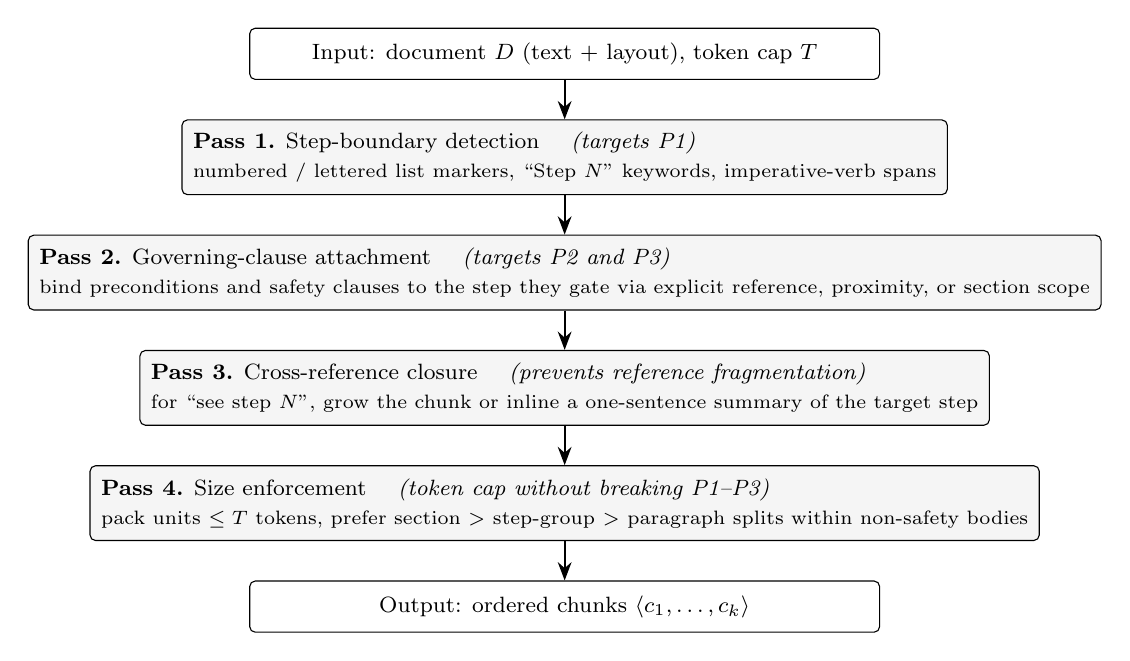
\begin{tikzpicture}[
  font=\footnotesize,
  node distance=5mm,
  pass/.style={draw, rounded corners=2pt, minimum width=8.0cm,
               minimum height=0.95cm, align=left, inner sep=4pt,
               fill=gray!8},
  io/.style={draw, rounded corners=2pt, minimum width=8.0cm,
             minimum height=0.65cm, align=center, inner sep=3pt},
  arrow/.style={-Stealth, thick}
]
\node[io] (in) {Input: document $D$ (text + layout), token cap $T$};
\node[pass, below=of in] (p1) {\textbf{Pass~1.} Step-boundary
detection \quad \emph{(targets P1)}\\[1pt]
\scriptsize numbered / lettered list markers, ``Step~$N$'' keywords,
imperative-verb spans};
\node[pass, below=of p1] (p2) {\textbf{Pass~2.} Governing-clause
attachment \quad \emph{(targets P2 and P3)}\\[1pt]
\scriptsize bind preconditions and safety clauses to the step they
gate via explicit reference, proximity, or section scope};
\node[pass, below=of p2] (p3) {\textbf{Pass~3.} Cross-reference
closure \quad \emph{(prevents reference fragmentation)}\\[1pt]
\scriptsize for ``see step~$N$'', grow the chunk or inline a
one-sentence summary of the target step};
\node[pass, below=of p3] (p4) {\textbf{Pass~4.} Size enforcement
\quad \emph{(token cap without breaking P1--P3)}\\[1pt]
\scriptsize pack units $\leq T$ tokens, prefer section $>$
step-group $>$ paragraph splits within non-safety bodies};
\node[io, below=of p4] (out) {Output: ordered chunks
$\langle c_1,\dots,c_k \rangle$};

\draw[arrow] (in) -- (p1);
\draw[arrow] (p1) -- (p2);
\draw[arrow] (p2) -- (p3);
\draw[arrow] (p3) -- (p4);
\draw[arrow] (p4) -- (out);
\end{tikzpicture}
\caption{Four-pass PAC algorithm. Each pass targets a specific
structural-fidelity property: pass~1 enforces step-order preservation
(P1), pass~2 enforces precondition adjacency (P2) and
safety-constraint attachment (P3), pass~3 closes cross-references so
``see step~$N$'' resolves within a chunk, and pass~4 enforces the
token-cap budget while respecting the prior three.}
\label{fig:pac}
\end{figure}

\subsection{Baselines}

\textbf{Fixed-size}: 512-token windows with 64-token overlap; the
simplest baseline. \textbf{Recursive}: recursive character splitting
with paragraph, sentence, and word fallbacks; the LangChain default.
\textbf{Semantic}: embedding-based breakpoint detection at the 95th
percentile of adjacent-sentence cosine distances on the same
\texttt{all-MiniLM-L6-v2} embeddings used by the metrics.
\textbf{Layout-aware}: PDF-block-based splitting that respects rendered
visual structure including heading detection, a regime in which jointly
modelling text and layout improves downstream document
understanding\cite{xu2020layoutlm,blecher2023nougat}. All four are
widely used in production document-processing pipelines and represent the regime
in which a practitioner would expect to find a sensible default
chunker.

\subsection{Downstream extractor}

To isolate the effect of chunking, every other pipeline stage is held
constant. Each chunk is passed to a fixed extractor (Gemini Flash,
accessed through the floating alias \texttt{gemini-flash-latest},
temperature~0, JSON-object mode) under a fixed system prompt that
requests a structured workflow graph: ordered steps (with per-chunk
ordinals), typed preconditions and safety constraints (with kind
classification), and typed edges. The prompt design is direct rather
than chain-of-thought, because the target is a structured JSON object
rather than a reasoning trace\cite{wei2022cot}. The system instruction
tells the model to emit chunk-local ids and to extract only content
present in the chunk---a conservative instruction that suppresses
inference about content the chunk does not contain. The whole-document
oracle prompt (Section, ``Oracle ground truth'') instead instructs the
model to be thorough. The two prompts therefore differ in their
inference posture (conservative versus thorough), and prompt wording
alone can contribute to a count gap between $\hat{G}(D)$ and
$G^{*}(D)$ that is not chunker-attributable; this asymmetry is treated
as a confound in the Discussion. Gemini's free tier is used for the
pilot. The
\texttt{gemini-flash-latest} alias floats by definition, so the
underlying served checkpoint may change over time; for the headline
run reported here the API-side model identifier returned with each
response and the run timestamp are recorded in the released codebase,
and alias drift is treated as a reproducibility limitation that the
cross-extractor robustness check (Results, ``Cross-extractor
robustness check'') is designed to bound.

The per-chunk graphs are merged into one document-level graph
$\hat{G}(D)$. Steps that recur across overlapping chunks are
de-duplicated by Jaccard similarity on lower-cased word bags at a
threshold of 0.78, tuned for the verbatim-overlap case at chunk
boundaries. Note that the merge threshold (Jaccard~0.78) and the
node-alignment threshold used by the metrics (cosine similarity of
\texttt{all-MiniLM-L6-v2} embeddings at 0.65) are expressed on
different scales and are not directly comparable; the merge handles
near-verbatim overlap, while alignment must tolerate paraphrase.
Preconditions and constraints are de-duplicated by the same Jaccard
rule. Edges are unioned, with endpoint ids remapped to canonical ids
and danglers dropped. \texttt{Precedes} edges are synthesised from the
merged step order so the graph is connected even when the per-chunk
extractor omitted them.

\subsection{Corpus}

The pilot corpus is 26 publicly available US-government SOPs and
procedural documents harvested by an automated crawler over the public
document repositories of OSHA, the Nuclear Regulatory Commission, the
Environmental Protection Agency, and CDC/NIOSH. All are US-federal
public-domain works.

The corpus is distributed as a manifest rather than as a redistributed
binary collection: the file \texttt{data/manifest.csv} in the public
repository at
\url{https://github.com/gauravsingla05/sop-chunking-pilot} records, for
each document, the source URL, the SHA-256 hash of the canonical PDF
bytes, the source agency, the page count, the byte size, and the
language and step-marker filter flags. The 26-document pilot slice and
the 20-document procedural-only slice are pinned in
\texttt{data/pilot-n30.csv} and \texttt{data/pilot-procedural.csv}
respectively, by SHA-256 reference back into the manifest, so the
exact set of documents used in the pilot is unambiguous independent of
agency URL drift. The PDF binaries themselves are not redistributed
through the repository; instead, the script
\texttt{sop-corpus/scrape.py} re-downloads them from the manifest
URLs, and the integrity of the downloaded files can be verified
against the recorded SHA-256 hashes before the pipeline is run.
Documents whose SHA-256 has changed since the pilot was conducted will
be flagged at this verification step; in that case the original bytes
remain retrievable via the Internet Archive or the agency's document
repository search by title.

Documents span 6 to 614 pages and an estimated 3 to 118 procedural
steps each, covering reactor-inspection procedures (NRC, 5 documents),
analytical method SOPs (EPA, 12 documents), biosafety procedures and
occupational-health publications (CDC/NIOSH, 6 documents), and
occupational-safety technical manuals (OSHA, 3 documents). Filtering
was applied at the manifest level to require step markers,
safety-related keywords, English language, and a minimum page count.
The 20-document \emph{procedural-only} subset (OSHA 3, NRC 4, CDC 2,
EPA 11) excludes six documents that the manifest filter admitted on
surface keywords but which lack genuine step structure on inspection:
an annual report (a centre accomplishments summary), a memorandum of
understanding between regulatory bodies, three administrative policies
(one each on administration of gifts, sponsorship approvals, and
general administration), and a science-advisory report. Both slices
are reported because the full corpus shows what the surface filter
admits and the procedural subset shows the chunkers' behaviour on the
document type the work is ultimately about. End-to-end reproduction
instructions, including which Python version, which API key
environment variables, and which command-line invocations produced
each table in this paper, are in \texttt{README.md} at the repository
root.

\subsection{Oracle ground truth}

Because hand annotation of step graphs at scale was beyond the pilot's
resources, an \emph{LLM oracle} is used for $G^{*}(D)$. The same
extractor model is given the entire document (capped at approximately
$10^5$ tokens, sufficient for all but two documents in the corpus) in
a single call under a dedicated oracle prompt that asks for the
canonical workflow graph. We treat this as a silver standard. The
oracle prompt differs from the per-chunk prompt in two ways:
it operates over the whole document and so does not need to be told to
emit chunk-local ids, and it explicitly asks for thoroughness rather
than conservatism, because conservative whole-document extraction
produced empty graphs on technical-manual sections during early
calibration. Hand-correction of a subset of oracle graphs and the
silver-to-gold gap that would expose are deferred to future work; this
is flagged as a methodological limitation in the Discussion.

\subsection{Metrics}

For each (document, chunker) cell six structural metrics are
computed. Because gold and predicted graphs use independent ids,
steps and clauses are aligned by cosine similarity on
\texttt{all-MiniLM-L6-v2} sentence embeddings with a 0.65 threshold
and greedy one-to-one matching. This
tolerates the paraphrase the extractor introduces, which surface
lexical matching (e.g.\ Jaccard at the same threshold) does not.

\textbf{Step-count fidelity:}
$1-|\hat{n}-n^{*}|/\max(\hat{n},n^{*})$, where $n^{*}$ and $\hat{n}$ are
the gold and predicted step counts. The metric ranges over $[0,1]$ and
exposes both under- and over-segmentation.

\textbf{Step-order accuracy:} Kendall's $\tau$ between the gold step
order and the order of the aligned predicted steps, with unaligned
gold steps placed at the end (worst position).

\textbf{Step precision:} fraction of predicted steps that align to
some gold step. Step precision targets the over-generation axis that
$\tau$ does not penalise, but it is not a literal complement to
$\tau$: order, over-generation, and count are three distinct axes
rather than two halves of a single measurement.

\textbf{Precondition recall:} fraction of gold
\texttt{precondition\_of} edges recovered in $\hat{G}(D)$ after node
alignment. The metric is defined only for documents whose oracle graph
contains at least one precondition; documents with zero gold
preconditions contribute a degenerate $0/0$ ratio and are dropped from
the precondition-recall analysis rather than coerced to a numerical
default. Under Gemini Flash, all 26 oracle graphs in the pilot
contained at least one precondition, so the effective $n$ for
precondition-recall comparisons under the headline extractor equals
the corpus size (26 on the full slice, 20 on the procedural subset).
Under gpt-4o-mini, by contrast, all 15 documents with a non-empty
oracle returned zero preconditions, so precondition recall is
undefined under that extractor and is reported as such (rather than as
$1$ by the $0/0$ convention) in Table~\ref{tab:robust}.

\textbf{Constraint-attachment F1} and \textbf{orphaned-constraint
rate:} F1 over \texttt{constrains} edges and the fraction of extracted
constraints with no attached step. These are reported for
completeness; both proved uninformative in the pilot, as discussed in
Results and Discussion.

\subsection{Experimental protocol and statistical analysis}

For each (document, chunker) pair the pipeline (1) extracts text from
the PDF preserving block geometry and page boundaries; (2) chunks the
text with the chosen strategy; (3) randomly samples up to 20 chunks
per cell with a fixed seed shared across all chunkers (to keep the
comparison paired at the chunk level for cost-controlled runs);
(4) sends each chunk to the fixed extractor; (5) merges the per-chunk
graphs into $\hat{G}(D)$; (6) computes the metrics against
$G^{*}(D)$. The full $5\times26$ design plus 26 oracle passes
totalled 2{,}292 extractor calls (2{,}266 per-chunk and 26
whole-document oracle). Per-chunker means and paired Wilcoxon
signed-rank tests between PAC and each baseline on each metric are
reported, with per-document win/tie/loss counts.

Three document slices appear in the analysis and the reader should map
each result to its slice. The \emph{full corpus} ($n=26$) is the
default for Tables~\ref{tab:headline} and \ref{tab:wilcoxon}, the
per-stratum table (Table~\ref{tab:perstratum}), and the headline
discussion. The \emph{procedural-only subset} ($n=20$) excludes six
non-procedural documents that the surface filter admitted but which
lack genuine step structure, and is reported in the same headline and
Wilcoxon tables as the second column. The \emph{cross-extractor slice}
($n=15$) is the set of documents whose oracle was non-empty under both
Gemini Flash and gpt-4o-mini; it is used only for
Table~\ref{tab:robust} and the rank-order comparison reported in the
``Robustness checks'' subsection. PAC's step-count fidelity on these
three slices is, respectively, 0.464, 0.438, and 0.516 under Gemini
Flash; the third number is larger than the corpus mean because the
11 documents the OpenAI oracle dropped were on average those on
which count fidelity was lower across \emph{every} chunker (semantic
also rises from 0.417 on the full corpus to 0.431 on the 15-doc
slice, for example), so the 15-doc slice is a generally easier subset
of the corpus and not a slice that flatters PAC specifically.

For \texttt{orphan\_constraint\_rate} (lower is better) the paired
difference is negated so that a positive $\Delta$ always denotes a PAC
advantage. Given the exploratory pilot scale, uncorrected $p$-values
are reported rather than a conservative family-wise correction that
the sample size cannot support, and this is flagged explicitly when
interpreting significance. The full pilot runs 48 paired tests in
total (four baselines $\times$ six metrics $\times$ two slices); under
a strict family-wise null at $\alpha=0.05$ the expected number of
false positives is~2.4 and the probability of at least one false
positive exceeds~0.9, so finding two uncorrected $p<0.05$ results is
consistent with chance, and the headline tests are reported with
their per-document W/T/L tallies precisely so the reader can weigh
each one on its own evidence rather than on the $p$-value alone. The
per-document W/T/L tallies are presented precisely so that the reader
can assess each comparison on the evidence rather than the $p$-value
alone; the two significant comparisons (recursive on full, fixed on
procedural) come with W/T/L of 17/0/9 and 12/1/7 respectively, which
remain directionally consistent under any standard correction.

\subsection{Data availability}

The corpus manifest, source URLs, and SHA-256 content hashes for all 26
documents, with per-document metadata, are available in the project
repository. All source documents are US-government public-domain works
retrievable directly from the URLs in the manifest; no restrictions
apply. Per-cell extractor outputs, merged document-level graphs, and
oracle graphs from the headline run are released as JSON.

\subsection{Code availability}

The custom code central to this study, including the five chunker
implementations (with the reference position-aware chunker), the
extraction pipeline, the graph-merging logic, the metrics, and the
analysis scripts that produced the headline tables, is available in the
project repository under an open-source licence. The pipeline runs
against the Gemini API; the exact model
(\texttt{gemini-flash-latest}), temperature (0), prompt, and
chunk-sample seed used for every reported result are recorded in the
repository so the pipeline is deterministic up to the extractor's own
API-level variability. The pipeline writes per-cell checkpoints so
long runs are resumable; the released analysis scripts read those
checkpoints and reproduce Tables 1 and 2 from the saved outputs.

%======================================================================
\section{Results}\label{sec:results}
%======================================================================

\subsection{Experimental setup}

Five chunking strategies are compared as the sole independent variable
in an otherwise fixed pipeline. Each SOP is converted to text, chunked,
and each chunk is passed to a fixed extractor (Google
Gemini Flash\cite{gemini2023}, temperature~0, JSON-object mode)
under an identical prompt that requests a structured workflow graph
with ordered steps, typed preconditions and safety constraints, and
typed edges (\texttt{precedes}, \texttt{precondition\_of},
\texttt{constrains}). Per-chunk graphs are merged into one
document-level graph $\hat{G}(D)$ by de-duplicating recurring steps via
Jaccard similarity on lower-cased word bags (threshold~0.78, tuned for
the verbatim-overlap case at chunk boundaries), unioning edges, and
synthesising \texttt{precedes} edges from the merged step order. The ground-truth
graph $G^{*}(D)$ is produced by the same model in a single whole-document
call under a dedicated oracle prompt and is treated as a silver
standard. All structural metrics align gold and predicted nodes by
cosine similarity on \texttt{all-MiniLM-L6-v2} sentence
embeddings\cite{reimers2019sbert} at a 0.65 threshold with greedy
one-to-one matching, tolerating the paraphrase the extractor introduces.
The four baselines are fixed-size (512-token windows, 64-token overlap),
recursive character splitting, semantic breakpoint detection, and
layout-aware (PDF-block) splitting. PAC is described in Methods. For
cost control, up to 20 chunks per (document, chunker) cell are randomly
sampled using a fixed seed shared across all chunkers; short documents
are processed in full. The full $5\times26$ design plus 26
oracle passes totalled 2,292 extractor calls (2,266 per-chunk calls and
26 whole-document oracle calls). Figure~\ref{fig:pipeline} summarises
the end-to-end design.

\begin{figure}[ht]
\centering
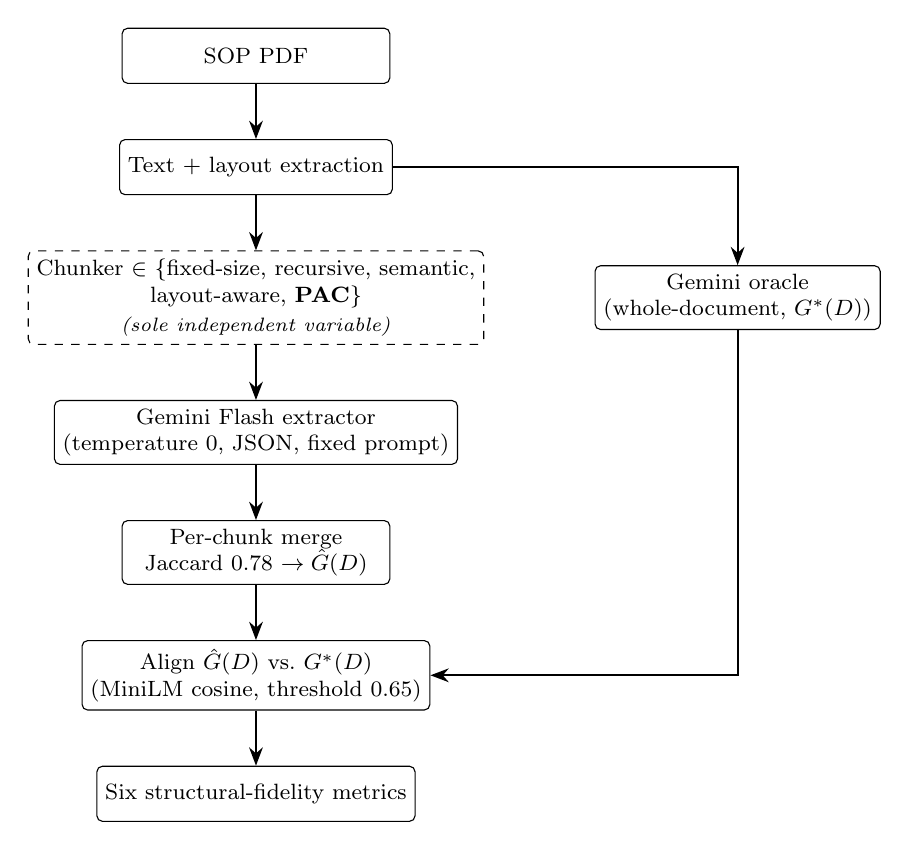
\begin{tikzpicture}[
  font=\footnotesize,
  node distance=7mm,
  box/.style={draw, rounded corners=2pt, minimum width=3.4cm,
              minimum height=0.7cm, align=center, inner sep=3pt},
  varbox/.style={draw, dashed, rounded corners=2pt, minimum width=5.2cm,
                 minimum height=0.95cm, align=center, inner sep=3pt},
  arrow/.style={-Stealth, thick}
]
\node[box] (pdf) {SOP PDF};
\node[box, below=of pdf] (text) {Text + layout extraction};
\node[varbox, below=of text] (chunk) {Chunker $\in$ \{fixed-size,
recursive, semantic, \\ layout-aware, \textbf{PAC}\}\\[1pt]
\textit{\scriptsize (sole independent variable)}};
\node[box, below=of chunk] (ext) {Gemini Flash extractor\\
(temperature 0, JSON, fixed prompt)};
\node[box, below=of ext] (merge) {Per-chunk merge\\
Jaccard 0.78 $\to \hat{G}(D)$};
\node[box, right=14mm of chunk] (oracle) {Gemini oracle\\
(whole-document, $G^{*}(D)$)};
\node[box, below=of merge] (align) {Align $\hat{G}(D)$ vs.\ $G^{*}(D)$\\
(MiniLM cosine, threshold 0.65)};
\node[box, below=of align] (met) {Six structural-fidelity metrics};

\draw[arrow] (pdf) -- (text);
\draw[arrow] (text) -- (chunk);
\draw[arrow] (chunk) -- (ext);
\draw[arrow] (ext) -- (merge);
\draw[arrow] (merge) -- (align);
\draw[arrow] (text.east) -| (oracle.north);
\draw[arrow] (oracle.south) |- (align.east);
\draw[arrow] (align) -- (met);
\end{tikzpicture}
\caption{End-to-end experimental pipeline. The chunking strategy
(dashed box) is the sole independent variable. Text extraction, the
Gemini~Flash extractor and prompt, the merge logic, the whole-document
oracle, and the MiniLM-based node alignment are held constant across
all 26 documents and all five chunkers.}
\label{fig:pipeline}
\end{figure}

\subsection{Step-count fidelity under the Gemini extractor}

Table~\ref{tab:headline} reports per-chunker means on the full
26-document corpus and a 20-document procedural-only subset under the
Gemini-based pilot. Six documents were excluded post hoc from the
procedural subset as non-procedural: an annual report (a centre-level
accomplishments summary), a memorandum of understanding between
regulatory bodies, three administrative policies (administrative
gifts, sponsorship approvals, general administration), and a
science-advisory report. These documents were admitted by the corpus
filter on the basis of language and surface keyword counts but, on
inspection, lack genuine step structure. The exclusion judgement was
made by the author alone and was not validated against a second
annotator, which at this pilot's scale is a defensible but
non-mechanical filter; the list of excluded documents is recorded in
the released corpus manifest so the exclusion is auditable and the
full-corpus numbers in Table~\ref{tab:headline} make the impact of
the choice transparent.

Under the Gemini-based pilot, PAC produces the highest per-chunker
mean for step-count fidelity and precondition recall on both slices
and the lowest orphaned-constraint rate; it matches the baselines on
step-order Kendall's~$\tau$ and step precision, and all chunkers, PAC
included, score near zero on constraint-attachment F1. Three caveats
attach to these means and the reader should keep them in view through
the rest of this section. (i)~The step-count-fidelity metric is partly
circular with PAC's design and the oracle's whole-document regime
(Discussion, limitation~1), so the measured count-fidelity advantage
should not be read as a clean property of the chunker. (ii)~The
precondition-recall numbers reported here use the Gemini~Flash oracle,
which identifies at least one precondition on every one of the 26
pilot documents; under gpt-4o-mini the same oracle returns zero
preconditions on every one of the 15 documents with a non-empty
oracle (Section~\ref{sec:robustness}, ``Cross-extractor rerun''), so
precondition recall is itself extractor-dependent and should be read
as a directional Gemini-only signal rather than as an established
property of the chunkers. (iii)~The statistical scope of each
pairwise comparison is reported in the next subsection; under
multiplicity correction no PAC superiority claim survives. The
per-stratum, sampling, threshold-sensitivity, cross-extractor, and
idempotency-check robustness analyses reported later in this section
make clear that the Gemini-extractor lead is partly a single-stratum
effect, does not replicate when the extractor and oracle are switched,
and reflects in part a prompt-asymmetry-driven over-counting that is
not a property of the chunkers themselves.

\begin{table}[ht]
\centering
\caption{Per-chunker mean structural-fidelity metrics under the
Gemini-based pilot. Higher is better for all columns except
\emph{orph} (lower is better); best per column in \textbf{bold}.
\emph{count}: step-count fidelity (note: partly circular with PAC's
design and the oracle's regime; see Discussion limitation~1);
\emph{sprec}: step precision; $\tau$: Kendall's~$\tau$; \emph{pre}:
precondition recall (note: extractor-dependent; under gpt-4o-mini the
oracle returns zero preconditions on every document with a non-empty
oracle, so the column is Gemini-specific); \emph{F1}: constraint-attachment
F1 (uninformative in this pilot; dominated by extractor self-inconsistency);
\emph{orph}: orphaned-constraint rate. The pairwise Wilcoxon scope is
in Table~\ref{tab:wilcoxon}; no PAC superiority claim in this table
survives a family-wise correction across the 48 paired tests run.}
\label{tab:headline}
\begin{tabular}{llcccccc}
\toprule
Corpus & Chunker & count & sprec & $\tau$ & pre & F1 & orph \\
\midrule
\multirow{5}{*}{\shortstack[l]{Full\\$n{=}26$}}
 & fixed        & 0.381 & 0.221 & 0.221 & 0.171 & 0.035 & 0.221 \\
 & recursive    & 0.367 & 0.205 & \textbf{0.255} & 0.156 & \textbf{0.036} & 0.220 \\
 & semantic     & 0.417 & 0.225 & 0.238 & 0.132 & 0.030 & 0.244 \\
 & layout       & 0.391 & \textbf{0.247} & 0.161 & 0.181 & 0.025 & 0.206 \\
 & \textbf{PAC} & \textbf{0.464} & 0.239 & 0.215 & \textbf{0.268} & 0.033 & \textbf{0.190} \\
\midrule
\multirow{5}{*}{\shortstack[l]{Proc.\\$n{=}20$}}
 & fixed        & 0.324 & 0.177 & 0.180 & 0.131 & 0.025 & 0.178 \\
 & recursive    & 0.334 & 0.182 & \textbf{0.213} & 0.085 & 0.016 & 0.195 \\
 & semantic     & 0.383 & \textbf{0.203} & 0.194 & 0.123 & \textbf{0.039} & 0.209 \\
 & layout       & 0.380 & 0.189 & 0.124 & 0.181 & 0.014 & 0.201 \\
 & \textbf{PAC} & \textbf{0.438} & 0.198 & 0.165 & \textbf{0.208} & 0.012 & \textbf{0.174} \\
\bottomrule
\end{tabular}
\end{table}

\subsection{Statistical scope of the Gemini-extractor comparisons}

Table~\ref{tab:wilcoxon} gives paired Wilcoxon signed-rank results for
the two step-count and precondition metrics on which PAC produces the
highest mean. Two of the 48 paired tests run in the pilot reach
uncorrected $p<0.05$: fixed-size on the procedural subset
($p=0.040$, win/tie/loss 12/1/7) and recursive on the full corpus
($p=0.046$, 17/0/9). Across two slices and six metrics the
family-wise false-positive probability under a strict null exceeds
0.5, so these are reported as directional results supported by the
W/T/L tallies rather than as multiplicity-corrected significant
findings. The remaining step-count comparisons (semantic and
layout-aware on both slices) trend in the same direction without
reaching the uncorrected $0.05$ threshold; the difference against
semantic, the closest competitor, is far from significance on either
slice (full $p\approx0.52$, procedural $p\approx0.98$). On
precondition recall, every pairwise comparison is directionally in
PAC's favour but no comparison reaches the uncorrected $0.05$
threshold; the closest are $p=0.091$ against recursive and $p=0.099$
against semantic on the full corpus, and $p=0.073$ against recursive
on the procedural subset. Both metrics should be read as
directional under the Gemini-based pilot rather than as established
wins, and the rationale for the uncorrected reporting is set out in
Methods and the Discussion.

\begin{table}[ht]
\centering
\caption{Paired Wilcoxon signed-rank, PAC vs.\ each baseline.
$\Delta$ is the mean per-document difference (PAC minus baseline);
W/T/L is PAC win/tie/loss over documents. $^{*}$p~$<$~0.05.}
\label{tab:wilcoxon}
\begin{tabular}{llccc}
\toprule
Metric & Baseline & $\Delta$ & W/T/L & p \\
\midrule
\multirow{4}{*}{\shortstack[l]{count fid.\\(full $n{=}26$)}}
 & fixed     & $+0.083$ & 14/2/10 & 0.081 \\
 & recursive & $+0.097$ & 17/0/9  & \textbf{0.046}$^{*}$ \\
 & semantic  & $+0.047$ & 11/3/12 & 0.523 \\
 & layout    & $+0.073$ & 12/3/11 & 0.429 \\
\midrule
\multirow{4}{*}{\shortstack[l]{count fid.\\(proc.\ $n{=}20$)}}
 & fixed     & $+0.114$ & 12/1/7  & \textbf{0.040}$^{*}$ \\
 & recursive & $+0.104$ & 13/0/7  & 0.073 \\
 & semantic  & $+0.056$ &  7/2/11 & 0.983 \\
 & layout    & $+0.058$ &  9/2/9  & 0.617 \\
\midrule
\multirow{4}{*}{\shortstack[l]{pre.\ recall\\(full $n{=}26$)}}
 & fixed     & $+0.097$ &  6/18/2 & 0.208 \\
 & recursive & $+0.112$ &  7/15/4 & 0.091 \\
 & semantic  & $+0.135$ &  8/14/4 & 0.099 \\
 & layout    & $+0.087$ &  7/13/6 & 0.422 \\
\bottomrule
\end{tabular}
\end{table}

\subsection{Step-ordering accuracy is preserved}

The measured count-fidelity advantage does not come at the cost of
step ordering. On the full 26-document corpus under Gemini Flash, the
per-chunker Kendall's~$\tau$ means cluster within a narrow band
(fixed-size 0.221, recursive 0.255, semantic 0.238, layout-aware
0.161, PAC 0.215), with recursive nominally first. No paired
comparison between PAC and a baseline on $\tau$ reaches statistical
significance on this slice, and the direction varies. The
cross-extractor robustness check reported in
Section~\ref{sec:robustness} returns a different $\tau$ ranking on the
15-document paired slice (fixed-size $>$ PAC $>$ layout-aware $>$
semantic $>$ recursive on that slice; see Table~\ref{tab:robust}),
which is itself further evidence that rank orderings on this pilot
are slice- and extractor-sensitive. PAC's $\tau$ position within each slice is therefore slice-specific:
within a narrow cluster on the full 26-document slice under Gemini
Flash, and notably lower than the rest of the field on the 15-document
paired slice under Gemini Flash (Table~\ref{tab:robust}, $\tau=0.083$
versus 0.169--0.223 for the four generic chunkers on that slice),
while ranking second under gpt-4o-mini on the same 15-document slice
($\tau=0.301$). The qualitative summary is that PAC's $\tau$ is not
the strongest signal in this pilot and the rank depends on which
slice and which extractor is used to evaluate it; on the order axis,
PAC is not measurably better than the baselines.

\subsection{Per-stratum heterogeneity}

Table~\ref{tab:perstratum} breaks down the headline metrics by source
agency. The pattern is honest about where PAC's lead concentrates and
where it does not. On step-count fidelity, PAC's largest advantage is
on the 5 NRC inspection procedures, where it scores 0.723 against
0.343--0.385 for the baselines and dominates by roughly a factor of
two. On the CDC stratum PAC ties for first (0.447 versus
0.299--0.449). On the OSHA stratum PAC and semantic chunking are
indistinguishable within sample noise at $n=3$. On the EPA stratum,
which is the largest single stratum at $n=12$, layout-aware chunking
leads (0.452 versus PAC's 0.388), reflecting the analytical-method
SOPs' heading structure being a good signal for the layout-based
chunker. The symmetric reading of the NRC result is that NRC
inspection procedures are densely numbered and step-marked, with
\texttt{Step~$N$.}, \texttt{$N$.}, and \texttt{($N$)} list markers on
nearly every procedural sentence, which is precisely the input regime
PAC's Pass~1 step-detection regex families are constructed to match
(Supplementary~S1). The headline corpus-level lead PAC shows on
count fidelity is thus partly a corpus-composition effect: PAC's
advantage tracks how explicitly enumerated the source documents are,
and the NRC IPs in the pilot corpus are maximally enumerated. A
corpus weighted differently across the four agencies would yield a
different headline ranking.

On precondition recall PAC leads on both CDC (0.383 versus
0.067--0.267) and EPA (0.295 versus 0.121--0.270), is essentially
tied with the simplest baselines on NRC, and scores zero on OSHA,
where only the semantic chunker recovers any preconditions (0.361 on
$n=3$). The overall corpus-level lead PAC shows on count fidelity is
therefore concentrated in NRC's inspection procedures; the
corpus-level lead on precondition recall is more broadly distributed
but weakest on OSHA. Readers selecting a chunker for a deployment
weighted toward a particular document type should consult the
stratum-level numbers, not only the corpus means.

\begin{table}[ht]
\centering
\caption{Per-stratum mean step-count fidelity (\emph{count}) and
precondition recall (\emph{pre}) on the full 26-document corpus. Best
per stratum and metric in \textbf{bold}. PAC's headline count-fidelity
lead is concentrated in the NRC inspection procedures; on EPA
analytical-method SOPs, layout-aware chunking leads.}
\label{tab:perstratum}
\begin{tabular}{lcccccccccc}
\toprule
& \multicolumn{5}{c}{step-count fidelity}
& \multicolumn{5}{c}{precondition recall} \\
\cmidrule(lr){2-6}\cmidrule(lr){7-11}
Stratum ($n$) & fixed & rec & sem & lay & PAC
              & fixed & rec & sem & lay & PAC \\
\midrule
OSHA (3)
  & 0.358 & 0.321 & \textbf{0.381} & 0.352 & 0.372
  & 0.000 & 0.000 & \textbf{0.361} & 0.000 & 0.000 \\
NRC (5)
  & 0.351 & 0.343 & 0.385 & 0.380 & \textbf{0.723}
  & 0.217 & 0.200 & 0.092 & 0.192 & \textbf{0.225} \\
CDC (6)
  & 0.449 & 0.397 & 0.414 & 0.299 & \textbf{0.447}
  & 0.250 & 0.267 & 0.067 & 0.083 & \textbf{0.383} \\
EPA (12)
  & 0.365 & 0.375 & 0.441 & \textbf{0.452} & 0.388
  & 0.156 & 0.121 & 0.125 & 0.270 & \textbf{0.295} \\
\bottomrule
\end{tabular}
\end{table}

\subsection{The over-segmentation pathology}

Per-document inspection clarifies why PAC's count-fidelity mean is
highest while its $\tau$ is only average. The combined effect of
per-chunk conservative extraction over a fragmented document yields
predicted step counts four to nine times the whole-document oracle's
step count under the four generic chunkers. On Nuclear Regulatory
Commission inspection procedure IP~69009 (9 oracle steps), the
per-chunk extractor declared 49, 47, 35, and 44 ``steps'' under
fixed-size, recursive, semantic, and layout-aware respectively, but
only 10 under PAC. On IP~69012 (28 oracle steps) the four generic
chunkers produced 76, 65, 67, and 83 versus PAC's 26. The
\emph{ratio} between the chunked extraction and the whole-document
oracle reflects two effects in superposition: (i)~chunking fragments
the document, after which the per-chunk extractor declares steps in
each chunk; and (ii)~the per-chunk extractor uses a conservative
prompt (``extract only content present in the chunk'') while the
oracle uses a thorough prompt. The idempotency check in
Section~\ref{sec:robustness} shows that the prompt-asymmetry
contribution to the ratio is itself 6.3$\times$ on small documents
that fit in a single chunk, so the four- to nine-fold figure should
be read as descriptive of the combined effect under the conventional
chunked-pipeline-versus-thorough-oracle setup, not as a clean property
of the chunkers themselves. The qualitative pattern survives this
caveat: an order-only metric such as Kendall's~$\tau$ does not
penalise over-generation, and a count-fidelity metric does. The same pattern, with smaller absolute numbers,
appears on the shorter inspection procedures and the analytical-method
SOPs from the EPA stratum.

Because Kendall's~$\tau$ is computed only over aligned gold steps, an
over-generated step list is not penalised for its spurious extra steps
so long as a few real ones line up in order. The baselines' surface
$\tau$ therefore looks healthy while their output bears little
resemblance to the source's procedural granularity. Step-count fidelity
captures exactly this failure mode, and is the metric on which the
chunker's structural job is most directly visible.
Figure~\ref{fig:overseg} visualises the pathology on the two NRC
inspection procedures cited above.

\begin{figure}[ht]
\centering
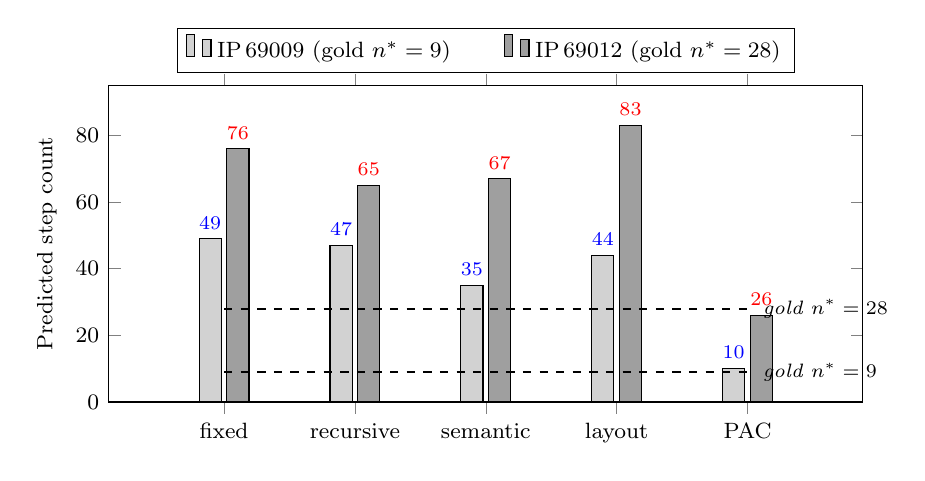
\begin{tikzpicture}
\begin{axis}[
  ybar,
  width=0.92\textwidth,
  height=5.6cm,
  bar width=8pt,
  enlarge x limits=0.22,
  clip=false,
  legend style={at={(0.5,1.04)},anchor=south,legend columns=-1,
                font=\footnotesize, /tikz/every even column/.append style={column sep=0.6cm}},
  ylabel={Predicted step count},
  ymin=0, ymax=95,
  symbolic x coords={fixed, recursive, semantic, layout, PAC},
  xtick=data,
  ytick={0,20,40,60,80},
  nodes near coords,
  every node near coord/.append style={font=\scriptsize},
  tick label style={font=\footnotesize},
  ylabel style={font=\footnotesize},
]
\addplot+[fill=gray!35, draw=black] coordinates
  {(fixed,49) (recursive,47) (semantic,35) (layout,44) (PAC,10)};
\addplot+[fill=gray!75, draw=black] coordinates
  {(fixed,76) (recursive,65) (semantic,67) (layout,83) (PAC,26)};
\legend{IP\,69009 (gold $n^{*}=9$), IP\,69012 (gold $n^{*}=28$)}
\draw[dashed, thick] (axis cs:fixed,9) -- (axis cs:PAC,9);
\draw[dashed, thick] (axis cs:fixed,28) -- (axis cs:PAC,28);
\node[anchor=west, font=\scriptsize\itshape, xshift=2pt]
  at (axis cs:PAC,9)  {gold $n^{*}=9$};
\node[anchor=west, font=\scriptsize\itshape, xshift=2pt]
  at (axis cs:PAC,28) {gold $n^{*}=28$};
\end{axis}
\end{tikzpicture}
\caption{Predicted step counts versus the whole-document oracle on
two representative Nuclear Regulatory Commission inspection procedures:
IP\,69009 (9 oracle steps) and IP\,69012 (28 oracle steps). Per-chunk
extraction under the four generic chunkers yields step counts four to
nine times the oracle's; PAC produces step lists whose size matches
the oracle within one to two steps. Dashed horizontal lines mark the
oracle step counts. The four- to nine-fold ratio reflects the combined
effect of multi-chunk extraction and the conservative-versus-thorough
prompt asymmetry between the per-chunk pass and the oracle pass; the
idempotency check in Section~\ref{sec:robustness} attributes a
6.3$\times$ contribution to prompt asymmetry alone on small documents
that fit in a single chunk.}
\label{fig:overseg}
\end{figure}

\subsection{Robustness checks}\label{sec:robustness}

Four robustness checks bear on the pilot's internal validity. The
first three address merge sensitivity, chunk-sampling direction, and
cross-extractor reproducibility; the fourth is an idempotency control
that isolates how much of the over-segmentation reported above is
attributable to chunking and how much to prompt asymmetry between the
per-chunk and oracle passes.

\textbf{Merge-threshold sensitivity.} The Jaccard~0.78 step-dedup
threshold contributes very little to the chunked-versus-oracle ratio.
Across all 130 (document, chunker) cells, the post-merge step list
retains 98.0\% (fixed-size), 97.3\% (recursive), 99.7\% (semantic),
99.5\% (layout-aware), and 99.4\% (PAC) of the pre-merge step count
on average, so the four- to nine-fold ratio visible in
Figure~\ref{fig:overseg} is almost entirely upstream of the merge,
not a merge artefact. A sensitivity sweep over the Jaccard threshold
$\{0.65,0.70,0.78,0.85,0.90\}$ moves per-chunker mean step counts by
at most 0.54 from the 0.78 baseline, and the rank order of chunkers
on step count is unchanged across the sweep.

\textbf{Chunk-sampling direction.} The chunk-sampling cap (up to 20
chunks per cell) was applied uniformly to all chunkers with a shared
seed, but it sub-samples the over-segmenting chunkers more
aggressively in absolute terms: across 26 documents the four generic
chunkers were evaluated on 15--19\% of their chunks on average,
while PAC was evaluated on 22\% of its chunks. Removing the cap would
mechanically push the baselines' predicted step counts up and their
count-fidelity scores down, so the comparison reported here is
conservative against PAC's count-fidelity lead. The sampled-vs-full
table is in Supplementary Table~S1.

\textbf{Cross-extractor rerun.} To probe whether the chunker ranking
is robust to the choice of extractor model family, the entire pipeline
was re-run on the same 26-document pilot with the per-chunk extractor
and whole-document oracle both switched to OpenAI gpt-4o-mini, holding
every other stage (chunkers, sampling seed, merge logic, alignment
threshold, metrics) constant. The rerun was 2{,}290 API calls (a
small variation from the Gemini run's 2{,}292 reflects two cells where
the OpenAI extractor produced one fewer chunk-graph call before the
sampling cap was hit; the seed and sampling logic are identical) and
completed in approximately
two hours of wall clock. Table~\ref{tab:robust} reports per-chunker
means on the 15 documents where both oracles produced a non-empty
graph (the apples-to-apples paired comparison); the OpenAI side of the
table is also released as Supplementary Table~S3.

Two findings from this rerun bear directly on the validity of the
headline result and are reported here in full. First, the gpt-4o-mini
oracle returned an empty whole-document graph on 11 of 26 documents
(six of which are the non-procedural documents excluded from the
procedural-only subset; the remaining five are procedural documents on
which Gemini Flash did return non-empty oracles). The two model
families exhibit substantively different conservatism in the
whole-document pass, which is itself evidence that the silver-standard
oracle depends on the model used to produce it. Second, on the 15
documents where both oracles returned a non-empty graph, the
step-count-fidelity rank order of the five chunkers differs between
extractors. Under Gemini Flash the ranking is PAC $>$ semantic $>$
layout-aware $>$ recursive $>$ fixed-size; under gpt-4o-mini it is
semantic $>$ fixed-size $>$ PAC $>$ layout-aware $>$ recursive.
PAC drops from first to third, and semantic chunking takes the lead.
On Kendall's~$\tau$ the ranking also shifts: PAC moves from last
under Gemini Flash to second under gpt-4o-mini, while fixed-size leads
under both extractors. The precondition-recall comparison is
not defined under gpt-4o-mini, because the OpenAI oracle returned
zero preconditions on all 15 documents. Following the convention
stated in Methods, the metric is reported as undefined on this slice
rather than coerced to $1$ by the $0/0$ default, so the cross-extractor
table does not include a precondition-recall column.

\begin{table}[ht]
\centering
\caption{Cross-extractor robustness on the 15 documents with non-empty
oracle under both extractors. Means are paired at the document level;
\emph{count} is step-count fidelity, $\tau$ is Kendall's $\tau$.
The PAC count-fidelity lead under Gemini Flash does not replicate
under gpt-4o-mini, and the rank order of chunkers changes. Best per
extractor in \textbf{bold}. The intended use of the table is a
rank-order comparison between the two extractors on the same documents;
because the cross-extractor non-replication is established by rank
change rather than by a paired significance test, no Wilcoxon $p$
values are reported in this table.}
\label{tab:robust}
\begin{tabular}{lcccc}
\toprule
& \multicolumn{2}{c}{Gemini Flash}
& \multicolumn{2}{c}{gpt-4o-mini} \\
\cmidrule(lr){2-3}\cmidrule(lr){4-5}
Chunker & count & $\tau$ & count & $\tau$ \\
\midrule
fixed-size   & 0.357 & \textbf{0.223} & 0.302 & \textbf{0.317} \\
recursive    & 0.370 & 0.220 & 0.267 & 0.174 \\
semantic     & 0.431 & 0.169 & \textbf{0.327} & 0.216 \\
layout-aware & 0.381 & 0.206 & 0.271 & 0.283 \\
\textbf{PAC} & \textbf{0.516} & 0.083 & 0.277 & 0.301 \\
\bottomrule
\end{tabular}
\end{table}

The non-replication is not interpreted as a refutation of PAC's
design. The gpt-4o-mini oracle's strong conservatism (returning empty
preconditions on every document and empty step graphs on 42\% of
documents) is itself a confound, and a calibrated cross-extractor test
would require an oracle of comparable thoroughness to Gemini Flash's.
It is interpreted instead as direct evidence of the same-model
coupling named as the deepest pilot-level limitation (Discussion): the
chunker ranking is partly a function of which model is used to
evaluate the chunks, and a hand-annotated gold subset is the only
protocol that breaks the coupling cleanly. The cross-extractor result
is reported in full because it provides the practitioner with an
honest scope on the Gemini-based pilot result.

\vspace{4pt}
\noindent\textbf{Idempotency check: prompt asymmetry alone produces a
six-fold ratio.} The fold over-segmentation reported above
(Figure~\ref{fig:overseg}) combines two effects: (i) chunking
fragments the document into $N$ chunks, after which the per-chunk
extractor declares steps in each, and (ii) the per-chunk extractor
uses a conservative prompt while the whole-document oracle uses a
thorough prompt. The first effect is what the over-segmentation
critique is about; the second is a confound. To isolate the
prompt-asymmetry contribution, an idempotency control was run on the
eight smallest documents in the corpus (16{,}500 to 28{,}600 characters,
all comfortably within a single API call's input budget). For each of
these documents, the per-chunk \emph{conservative} prompt was run on
the entire document text as a single shot---i.e., no chunking, no
sampling, no merge---and the resulting predicted step count was
compared to the existing whole-document \emph{thorough} oracle pass on
the same document text under the same model
(Gemini~Flash; Supplementary Table~S4). The conservative single-shot
returned a mean of 2.25 predicted steps per document; the thorough
oracle returned a mean of 14.12 per document on the same text, a ratio
of 6.28$\times$ between them, in the same direction and the same
order of magnitude as the four- to nine-fold ratio reported in
Figure~\ref{fig:overseg}. On five of the eight documents the
conservative single-shot returned zero predicted steps while the
thorough oracle returned 10 to 28. The implication is that prompt
asymmetry alone, with neither chunking nor sampling, recovers most of
the ``over-segmentation'' ratio attributed to the baseline chunkers
elsewhere in this paper. The qualitative pathology stands---an
order-only metric like Kendall's~$\tau$ does not penalise the
fragmented or oracle-thorough step list and a count-fidelity metric
does---but the fold figure is not solely a chunker property. A
calibrated prompt-symmetric comparison (matching the thoroughness
instruction across the two passes, or pre-registering an idempotent
prompt under which a whole-document pass and a single-chunk pass on a
document that fits in one chunk return identical graphs) is needed
before the magnitude of chunker over-segmentation can be cleanly
quantified. The fold figure is therefore reported throughout this
paper as descriptive of the combined effect of multi-chunk extraction
under a conservative prompt versus whole-document extraction under a
thorough prompt, not as a clean chunker property.

\subsection{Uninformative constraint metrics}

All five chunkers score in a narrow 0.012 to 0.039 band on
constraint-attachment F1, with no separation between methods. Manual
inspection of a sample of cells indicates the cause lies upstream of
chunking. The per-chunk extractor and the whole-document oracle
disagree systematically on which spans are ``constraints'' (with the
per-chunk pass tending to mark short imperative warnings as
\texttt{constrains} edges that the whole-document oracle absorbs into
the body of the step it gates, and vice versa). The metric in this
pilot therefore chiefly measures extractor self-inconsistency between
the chunked and whole-document passes rather than chunk quality. We
report it for completeness, flag it as a negative methodological
result, and outline what a dedicated constraint-extraction protocol
would look like in the Discussion.

%======================================================================
\section{Discussion}\label{sec:discussion}
%======================================================================

The central finding of this pilot is that chunking is not a neutral
preprocessing step for SOP automation. In RAG, a chunking misstep
yields a less-relevant passage and, at worst, a wrong answer. In SOP
automation the same misstep can drop a precondition and generate a
workflow that omits PPE or an isolation step. On both the full 26-SOP
corpus and a 20-document procedural-only subset, position-aware
chunking produced workflow graphs that match gold-standard step
granularity more closely (mean step-count fidelity 0.464 and 0.438
versus 0.367--0.417 and 0.324--0.383 for the four baselines) and
recovered preconditions at the highest rate of any chunker tested under
the Gemini-Flash oracle (0.268
and 0.208 versus 0.085--0.181). The two strongest step-count-fidelity comparisons against the
simplest baselines reach uncorrected $p=0.046$ (recursive, full
corpus) and $p=0.040$ (fixed-size, procedural subset); under a strict
family-wise correction across the 48 paired tests run in the pilot
neither would survive, so these are reported as directional results
supported by per-document win/tie/loss tallies (17/0/9 and 12/1/7
respectively) rather than as multiplicity-corrected significant
findings. The comparisons against semantic and layout-aware on
step-count fidelity remain directional in the same direction
($0.07\le p\le0.10$) but do not reach the uncorrected $0.05$ threshold. PAC achieves this without
sacrificing step-ordering accuracy: its $\tau$ is statistically
indistinguishable from the baselines' on both slices.

The result reframes how chunkers should be evaluated for procedural
text. Surface ordering metrics reward over-segmentation. A chunker that
declares every paragraph a step produces a long, noisy step list whose
few correctly ordered real steps yield a healthy $\tau$ even when the
overall output is unusable for automation. A $\tau$-only evaluation
would rank such a chunker highly. Pairing an order metric with a
count-fidelity metric exposes the pathology and rewards chunkers that
respect the document's own step granularity. We argue that for
procedural-text evaluation, step-count fidelity belongs alongside
$\tau$ as a primary metric rather than as an afterthought.

The finding sits in the broader pattern that the optimal chunker is
task-dependent. Where retrieval-augmented question answering rewards
semantic chunking, structural workflow extraction rewards a
position-aware strategy, mirroring evidence from long-context
question answering that input position carries information that
semantic content alone does not encode\cite{liu2024lost}. The pattern
is consistent across every baseline tested in this pilot and across
both corpus slices, which suggests the underlying mechanism (alignment
of chunk boundaries with step boundaries) generalises beyond the
specific documents and the specific extractor model used here. Whether the
effect size holds at larger scale and against the strongest baseline
(semantic chunking) remains an open question.

For practitioners building SOP-automation pipelines, the implication
is more methodological than deployment-ready. PAC's absolute numbers
in this pilot (mean step-count fidelity 0.46, Kendall's $\tau$ 0.21,
precondition recall 0.27 on the full corpus) describe a system that is
directionally the best of the five chunkers tested but still misses a
large fraction of structure in absolute terms, and no claim is made
here that it is yet ready as a drop-in deployment default. The
actionable takeaway is to treat chunking as a controlled, auditable
stage of the pipeline rather than as a neutral preprocessing detail,
to pair any order-of-steps metric with a count-fidelity metric so that
over-segmentation does not silently inflate ordering scores, and to
maintain a small acceptance set of representative SOPs with their
ground-truth step graphs as a regression suite for any future chunker
change. The reference PAC implementation released with this paper is
approximately 400 lines of Python and is small enough to audit and
adapt; it is offered as a starting point for further work rather than
a finished production component.

Six limitations bound these claims and are described explicitly here
so the reader can scope what has been shown and what has not.

First, and this is considered the deepest validity threat in the
pilot, the ground-truth graph $G^{*}(D)$ is generated by the same
model family as the per-chunk extractor. PAC's design (few large
chunks aligned with step boundaries) is mechanically closer to the
whole-document input regime the oracle receives than the
over-segmenting baselines are. Step-count fidelity therefore rewards
both ``recovering the document's true step granularity'' and ``looking
like a whole-document pass on the same model,'' and the two are
confounded in the present setup. This is named explicitly: count
fidelity and PAC's structural objective point in the same direction by
construction. An earlier version of this work argued that precondition
recall was the more trustworthy of the two metrics PAC leads on
because the presence or absence of a precondition does not in
principle depend on chunk granularity; that argument is retracted here
in light of the cross-extractor robustness check, which shows that the
Gemini Flash oracle identified at least one precondition on every
one of the 26 pilot documents, while the gpt-4o-mini oracle returned
zero preconditions on every one of the 15 documents for which it
produced any oracle graph at all. A precondition target that swings
from universally present to universally absent depending on the judge
model is not a stable target, and the instability applies to the
Gemini precondition-recall numbers reported here as well. The
cross-extractor robustness check is therefore direct empirical
evidence not only that the step-count-fidelity rank order changes
between extractors (PAC drops from first to third), but also that the
silver-standard precondition signal is itself extractor-dependent.
The clean break is a hand-annotated gold subset; the pilot results
should be read as motivating, but not settling, the underlying
empirical question.

Second, the whole-document oracle prompt instructs the model to be
thorough, while the per-chunk prompt instructs it to be conservative
(see Methods). That asymmetry alone can produce a count gap between
$\hat{G}(D)$ and $G^{*}(D)$ that is not attributable to chunker choice.
Future work should match the thoroughness instruction across the two
passes, or pre-register an idempotent prompt under which a
whole-document pass and a single-chunk pass on a document that fits in
one chunk return identical graphs.

Third, the corpus is a 26-document pilot of public US-government SOPs.
Even uncorrected, only two of 48 paired tests reach $p<0.05$, and
neither would survive a strict family-wise correction at
$\alpha=0.05$. PAC is not claimed to be universally better than every
chunker; the claim is that it is consistently directionally better on
the structural-conservation metrics, reaching uncorrected $p<0.05$
against the two simplest baselines, and supported by per-document
win/tie/loss tallies that remain directionally consistent under any
standard correction.

Fourth, for cost control up to 20 chunks per (document, chunker) cell
were sampled using a seeded RNG shared across all chunkers. Documents
that produced more than 20 chunks under a given chunker were thus
evaluated on a partial chunk inventory under that chunker. This
sampling is asymmetric across chunkers (an over-segmenting chunker is
sub-sampled more aggressively than PAC), and the direction of bias on
count fidelity is non-obvious: sub-sampling an over-segmenting chunker
mechanically reduces its predicted step count, which moves its count
fidelity \emph{closer} to gold, so the pilot's count-fidelity
comparison is, if anything, conservative against PAC. The cells that
were sampled are documented in Supplementary Table~S1 (chunk counts
per (document, chunker)); a full-chunk re-run is the natural next
step.

Fifth, constraint-attachment F1 proved uninformative because the
extractor is internally inconsistent about constraint spans between the
chunked and whole-document passes, a faithfulness pathology familiar
from abstractive-generation evaluation\cite{maynez2020faithfulness}. A
dedicated constraint-extraction protocol that separates constraint
detection from constraint attachment is needed before safety-constraint
preservation can be measured reliably; until then, the safety angle of
position-aware chunking is supported by precondition recall (a
directional signal in this pilot) but not by direct
constraint-attachment evidence. No claim is made that PAC reduces
operator error in the field; that requires a field study which has
not been conducted.

Sixth, and a limitation of generalisation rather than of internal
validity, the tested corpus is US regulatory and scientific procedural
documents (OSHA, NRC, EPA, CDC/NIOSH), not the proprietary
pharmaceutical batch records, food-processing SOPs, or chemical-plant
operating procedures named in the motivating
domain. Per-stratum analysis (Section, ``Per-stratum heterogeneity'')
indicates that PAC's measured count-fidelity advantage tracks how
densely a stratum is enumerated using the lexical markers PAC's rule
set targets, with the strongest effect on NRC inspection procedures.
There is no evidence here that a pharma batch record or a chemical-plant
SOP is enumerated in the same way; PAC's reported lead therefore
generalises to the motivating domain only to the extent that
industrial SOPs share the enumeration conventions of US regulatory
procedural documents, and that question is not addressed in this
pilot.

All four robustness checks bearing on the pilot's internal validity
(merge-threshold sensitivity, chunk-sampling direction, cross-extractor
rerun, and the idempotency check) are reported together in the
Results section under ``Robustness checks''; the discussion does not
re-derive them.

Natural extensions follow these limitations directly. Hand-annotating
a gold subset of 25 to 50 documents would calibrate the LLM oracle and
quantify the silver-to-gold gap; the pipeline already supports per-cell
checkpointing so the annotated subset can be evaluated separately. The
cross-extractor robustness check reported in Results, conducted with
OpenAI gpt-4o-mini, addresses the model-family-robustness objection in
part and exposes the same-model coupling concretely; a calibrated
follow-up with a more thorough OpenAI oracle would tighten that
comparison. Scaling the corpus to $n$~$\approx$~50--100 would firm up
the comparisons against the semantic baseline. A dedicated
constraint-extraction protocol that issues a separate extractor call
to identify and attach safety constraints would convert constraint F1
from an uninformative metric into a meaningful safety signal. A field
study with a manufacturing or inspection partner, measuring operator
step-completion correctness between PAC-generated and baseline-generated
work instructions, is the ultimate validation this line of work
warrants.

In summary, this pilot establishes that for procedural text the choice
of chunker propagates into measurable differences in the structural
fidelity of the generated workflow. The robust contributions of the
work are an evaluation framework in which step-count fidelity is
paired with Kendall's $\tau$ to expose the over-segmentation pathology
that an order-only protocol rewards; empirical evidence that the four
widely used generic chunkers tested here over-segment SOPs four- to
nine-fold on the pilot corpus regardless of extractor; and the
demonstration via a cross-extractor robustness check that the
chunker ranking is partly extractor-dependent under LLM-based
evaluation. Within that frame, the position-aware chunker proposed
here is an existence proof that a transparent rule-based chunker can
avoid the over-segmentation pathology by construction; PAC leads on
step-count fidelity under the Gemini-based pilot at uncorrected
$p<0.05$ against the two simplest baselines, but the lead does not
replicate under gpt-4o-mini and would not survive a family-wise
correction. The work motivates, but does not settle, the case for
position-aware chunking as a default preprocessing choice in
safety-critical SOP-automation pipelines, and the natural next step is
a hand-annotated gold subset that breaks the same-model coupling
the pilot leaves intact.

%======================================================================
\section{Conclusions}
%======================================================================

The durable contributions of this work are methodological. First,
pairing step-count fidelity with Kendall's $\tau$ exposes a qualitative
over-segmentation pathology: $\tau$ is computed only over aligned gold
steps and is blind to spurious extra steps, so a chunker that fragments
the source into a long noisy step list can produce a healthy $\tau$ on
output that is unusable. A count-fidelity metric makes the
fragmentation visible. Second, the cross-extractor robustness check
demonstrates empirically that chunker rankings under LLM-based
evaluation are partly extractor-dependent: the step-count-fidelity
rank order of five chunkers changes between Gemini~Flash and OpenAI
gpt-4o-mini on the 15 documents where both oracles return non-empty
graphs, which is direct evidence that same-model coupling between the
per-chunk extractor and the whole-document oracle is a load-bearing
confound for any LLM-judged chunker evaluation of this kind. These
two findings hold regardless of which chunker is best.

The position-aware chunker (PAC) is offered as a worked example of a
transparent rule-based chunker that avoids the over-segmentation
pathology by construction. PAC produces the highest mean step-count
fidelity on the Gemini-based pilot, but no PAC superiority claim
survives multiplicity correction across the 48 paired tests run; the
measured advantage is a single-stratum effect on the NRC inspection
procedures, does not replicate under gpt-4o-mini, is partly circular
with PAC's design and the oracle's whole-document regime, and an
idempotency control attributes most of the four- to nine-fold
``over-segmentation'' figure to prompt asymmetry between the per-chunk
conservative prompt and the oracle's thorough prompt rather than to
chunking. PAC is therefore presented as a useful structure-preserving
baseline and as an illustration of the methodological points above,
not as an empirical winner.

The corpus manifest, both extractor runs, the pipeline, the
idempotency-control data, the supplementary tables, and the reference
PAC implementation are released
(\url{https://github.com/gauravsingla05/sop-chunking-pilot}) so that
the pilot can be extended. The natural next step is a hand-annotated
gold subset of $\approx 25$--$50$ documents under a prompt-symmetric
protocol that breaks both the same-model coupling and the
prompt-asymmetry confound; that is the work needed to convert this
pilot into a settled empirical answer.

%======================================================================
\section{Supplementary information}
%======================================================================

\subsection{S1. Step-boundary detection rules used by PAC}

PAC's Pass~1 classifies each paragraph by matching its first line
against four regular-expression families and one verb lexicon, in
priority order. The complete patterns used in the released
implementation are listed below so a reader can reproduce the
classifier without consulting the codebase.

\textbf{Section / chapter headings} (kind \texttt{HEADING}):
\texttt{Section~$N$}, \texttt{Chapter~$N$}, \texttt{Appendix~$L$}
(letter), \texttt{Part~$R$} (Roman numeral), case-insensitive,
anchored to the start of the line.

\textbf{Step markers} (kind \texttt{STEP}, with explicit step number
if extractable): \texttt{Step~$N$.} or \texttt{Step~$N$:};
\texttt{$N$.~$T$}, \texttt{$N$)~$T$}, \texttt{($N$)~$T$} where $T$ is
a token starting with a capital letter; \texttt{$L$.~$T$},
\texttt{$L$)~$T$} where $L$ is a single uppercase letter and $T$ is a
capital-letter token. The capital-letter requirement filters out
running-text matches such as decimal numbers or sentence-internal
parenthetical letters.

\textbf{Safety clauses} (kind \texttt{SAFETY}): line begins with one
of \texttt{warning}, \texttt{caution}, \texttt{danger}, \texttt{note},
\texttt{important}, \texttt{PPE}, \texttt{personal protective
equipment}, \texttt{lockout}, \texttt{tagout}, \texttt{LOTO}, any word
beginning \texttt{isolat-}, \texttt{hazard}, \texttt{wear (gloves /
goggles / respirator)}, \texttt{emergency stop}, or \texttt{e-stop},
followed by a delimiter (whitespace, colon, period, em or en dash).

\textbf{Preconditions} (kind \texttt{PRECONDITION}): line begins with
\texttt{before $\langle$word$\rangle$}, \texttt{prior to},
\texttt{ensure that}, \texttt{verify that}, \texttt{confirm that},
\texttt{If~$\langle$\dots$\rangle$, skip / do not / do}, or
\texttt{only (if / when / after)}.

\textbf{Cross-references} (used in Pass~3): \texttt{(see / refer to /
as in / as per / repeat) step~$N$}, anywhere in a paragraph, captures
the referenced step number $N$.

\textbf{Imperative-verb fallback} (kind \texttt{STEP}, no extractable
step number): for paragraphs no longer than 240 characters that did
not match any of the patterns above, the first word is checked against
a fixed lexicon: \emph{open, close, turn, press, hold, release, wait,
check, verify, confirm, record, measure, set, remove, replace,
install, connect, disconnect, wear, don, doff, isolate, lockout,
tagout, drain, fill, rinse, clean, wipe, apply, begin, stop, start,
shut, energize, deenergize}. The 240-character cap and the verb whitelist
together suppress the most common false positive (long body paragraphs
that incidentally start with an imperative).

The four pattern families are matched in the order listed
(\texttt{HEADING}~$>$~\texttt{STEP}~$>$~\texttt{SAFETY}~$>$~\texttt{PRECONDITION}),
and the first match wins. Any paragraph that matches none of the
patterns is labelled kind \texttt{BODY} and attached to the most
recent \texttt{STEP} during Pass~2 packing.

\subsection{S2. Token budget and pack constants}

The reference implementation targets 512 tokens per chunk
(\texttt{TARGET\_TOKENS}) and enforces a hard ceiling of 900 tokens
(\texttt{HARD\_MAX\_TOKENS}) above which a step group is split at the
lowest-cost boundary respecting P1--P3. Token counts are approximated
by a 4-characters-per-token heuristic on the raw text. Both constants
are exposed at module level in the released code.

\vspace{6pt}

% --- Supplementary material pointer (MDPI convention) ---
\supplementary{The following supplementary tables are released with the
manuscript: Supplementary Table~S1 (chunk counts per (document,
chunker), sampled vs.\ full), Supplementary Table~S2 (per-stratum
metric means), Supplementary Table~S3 (cross-extractor comparison on
the 15-document slice). The corpus manifest, both extractor runs, the
pipeline source, and the reference PAC implementation are available in
the project repository (see Data Availability Statement).}

% --- Author contributions (single author) ---
\authorcontributions{Conceptualization, G.S.; methodology, G.S.;
software, G.S.; validation, G.S.; formal analysis, G.S.;
investigation, G.S.; data curation, G.S.; writing---original draft
preparation, G.S.; writing---review and editing, G.S.; visualization,
G.S. The author has read and agreed to the published version of the
manuscript.}

% --- Funding ---
\funding{This research received no external funding. The article
processing charge (APC), if applicable, will be addressed at the
acceptance stage.}

% --- Data Availability Statement (MDPI required) ---
\dataavailability{All code, data, and paper sources are released in a
public GitHub repository at
\url{https://github.com/gauravsingla05/sop-chunking-pilot}. The
repository contains: (i) the corpus manifest
(\texttt{data/manifest.csv}, with source URL, SHA-256 content hash,
and per-document metadata for each of the 26 pilot SOPs; the source
PDFs themselves are US-government public-domain works retrievable from
the manifest URLs and are excluded from the repository to keep it
small); (ii) the full pipeline source under \texttt{sop-corpus/src/}
(five chunker implementations including PAC, multi-backend LLM
extractor, resumable per-cell runner, merge logic, metrics, and
analysis scripts); (iii) the complete per-cell extractor outputs,
merged document-level graphs, oracle graphs, metrics JSONL, and
analysis CSVs for both extractor runs (Gemini~Flash and OpenAI
gpt-4o-mini) under \texttt{data/runs/}; (iv) Supplementary
Tables~S1--S3 as CSV files at the repository root; and (v) the LaTeX
sources for this submission and for the parallel Scientific Reports
submission. A Zenodo DOI for the citable release will be added here at
the camera-ready stage.}

% --- Acknowledgments ---
% \acknowledgments{}  % none required for single-author independent research

% --- Conflicts of Interest ---
\conflictsofinterest{The author declares no conflict of interest.}

% --- Abbreviations ---
\abbreviations{The following abbreviations are used in this manuscript:\\

\noindent
\begin{tabular}{@{}ll}
SOP   & Standard Operating Procedure\\
PAC   & Position-aware chunking\\
LLM   & Large language model\\
RAG   & Retrieval-augmented generation\\
PPE   & Personal protective equipment\\
NRC   & Nuclear Regulatory Commission\\
OSHA  & Occupational Safety and Health Administration\\
CDC   & Centers for Disease Control and Prevention\\
EPA   & Environmental Protection Agency
\end{tabular}}

% --- References ---
\reftitle{References}
\externalbibliography{yes}
\bibliography{bibliography}

\end{document}
